\documentclass[a4paper]{article} %format de la feuille + type de document https://en.wikibooks.org/wiki/LaTeX/Document_Structure#Document_classes
%packages nécessaire pour nos besoins
\usepackage[utf8]{inputenc}
\usepackage[T1]{fontenc}
\usepackage[english,french]{babel}
\usepackage{amsmath}
\usepackage{amssymb,amsfonts,textcomp}
\usepackage{color}
\usepackage{array}
\usepackage{hhline}
\usepackage{hyperref}
\usepackage[pdftex]{graphicx}
\usepackage{sectsty}
\usepackage{tcolorbox}
\usepackage{textcomp}
\usepackage{courier}
\usepackage[font={small,it}]{caption}
\usepackage{float}
\usepackage{graphicx}
\usepackage{caption}
\usepackage{tabularx}
\usepackage{multirow}% http://ctan.org/pkg/multirow
\usepackage{tikz}
\usepackage[top=25mm,bottom=25mm,right=25mm,left=25mm]{geometry} 
\usepackage[export]{adjustbox}
\usepackage{listings}


%Définition des couleurs
\definecolor{havelockBlue}{rgb}{0.004, 0.42, 0.73}
\definecolor{Monokaimagenta}{rgb}{0.86,0.08,0.24}
\definecolor{codegray}{rgb}{0.5,0.5,0.5}
\definecolor{backcolour}{rgb}{0.95,0.95,0.92}

\lstdefinelanguage[mips]{Assembler}{%
  % so listings can detect directives and register names
  alsoletter={.\$},
  % strings, characters, and comments
  morestring=[b]",
  morestring=[b]',
  morecomment=[l]\#,
  % instructions
  morekeywords={[1]abs,abs.d,abs.s,add,add.d,add.s,addi,addiu,addu,%
    and,andi,b,bc1f,bc1t,beq,beqz,bge,bgeu,bgez,bgezal,bgt,bgtu,%
    bgtz,ble,bleu,blez,blt,bltu,bltz,bltzal,bne,bnez,break,c.eq.d,%
    c.eq.s,c.le.d,c.le.s,c.lt.d,c.lt.s,ceil.w.d,ceil.w.s,clo,clz,%
    cvt.d.s,cvt.d.w,cvt.s.d,cvt.s.w,cvt.w.d,cvt.w.s,div,div.d,div.s,%
    divu,eret,floor.w.d,floor.w.s,j,jal,jalr,jr,l.d,l.s,la,lb,lbu,%
    ld,ldc1,lh,lhu,li,ll,lui,lw,lwc1,lwl,lwr,madd,maddu,mfc0,mfc1,%
    mfc1.d,mfhi,mflo,mov.d,mov.s,move,movf,movf.d,movf.s,movn,movn.d,%
    movn.s,movt,movt.d,movt.s,movz,movz.d,movz.s,msub,msubu,mtc0,mtc1,%
    mtc1.d,mthi,mtlo,mul,mul.d,mul.s,mulo,mulou,mult,multu,mulu,neg,%
    neg.d,neg.s,negu,nop,nor,not,or,ori,rem,remu,rol,ror,round.w.d,%
    round.w.s,s.d,s.s,sb,sc,sd,sdc1,seq,sge,sgeu,sgt,sgtu,sh,sle,%
    sleu,sll,sllv,slt,slti,sltiu,sltu,sne,sqrt.d,sqrt.s,sra,srav,srl,%
    srlv,sub,sub.d,sub.s,subi,subiu,subu,sw,swc1,swl,swr,syscall,teq,%
    teqi,tge,tgei,tgeiu,tgeu,tlt,tlti,tltiu,tltu,tne,tnei,trunc.w.d,%
    trunc.w.s,ulh,ulhu,ulw,ush,usw,xor,xori},
  % assembler directives
  morekeywords={[2].align,.ascii,.asciiz,.byte,.data,.double,.extern,%
    .float,.globl,.half,.kdata,.ktext,.set,.space,.text,.word},
  % register names
  morekeywords={[3]\$0,\$1,\$2,\$3,\$4,\$5,\$6,\$7,\$8,\$9,\$10,\$11,%
    \$12,\$13,\$14,\$15,\$16,\$17,\$18,\$19,\$20,\$21,\$22,\$23,\$24,%
    \$25,\$26,\$27,\$28,\$29,\$30,\$31,%
    \$zero,\$at,\$v0,\$v1,\$a0,\$a1,\$a2,\$a3,\$t0,\$t1,\$t2,\$t3,\$t4,
    \$t5,\$t6,\$t7,\$s0,\$s1,\$s2,\$s3,\$s4,\$s5,\$s6,\$s7,\$t8,\$t9,%
    \$k0,\$k1,\$gp,\$sp,\$fp,\$ra},
    literate=
  {á}{{\'a}}1 {é}{{\'e}}1 {í}{{\'i}}1 {ó}{{\'o}}1 {ú}{{\'u}}1
  {Á}{{\'A}}1 {É}{{\'E}}1 {Í}{{\'I}}1 {Ó}{{\'O}}1 {Ú}{{\'U}}1
  {à}{{\`a}}1 {è}{{\`e}}1 {ì}{{\`i}}1 {ò}{{\`o}}1 {ù}{{\`u}}1
  {À}{{\`A}}1 {È}{{\'E}}1 {Ì}{{\`I}}1 {Ò}{{\`O}}1 {Ù}{{\`U}}1
  {ä}{{\"a}}1 {ë}{{\"e}}1 {ï}{{\"i}}1 {ö}{{\"o}}1 {ü}{{\"u}}1
  {Ä}{{\"A}}1 {Ë}{{\"E}}1 {Ï}{{\"I}}1 {Ö}{{\"O}}1 {Ü}{{\"U}}1
  {â}{{\^a}}1 {ê}{{\^e}}1 {î}{{\^i}}1 {ô}{{\^o}}1 {û}{{\^u}}1
  {Â}{{\^A}}1 {Ê}{{\^E}}1 {Î}{{\^I}}1 {Ô}{{\^O}}1 {Û}{{\^U}}1
  {œ}{{\oe}}1 {Œ}{{\OE}}1 {æ}{{\ae}}1 {Æ}{{\AE}}1 {ß}{{\ss}}1
  {ű}{{\H{u}}}1 {Ű}{{\H{U}}}1 {ő}{{\H{o}}}1 {Ő}{{\H{O}}}1
  {ç}{{\c c}}1 {Ç}{{\c C}}1 {ø}{{\o}}1 {å}{{\r a}}1 {Å}{{\r A}}1
  {€}{{\euro}}1 {£}{{\pounds}}1 {«}{{\guillemotleft}}1
  {»}{{\guillemotright}}1 {ñ}{{\~n}}1 {Ñ}{{\~N}}1 {¿}{{?`}}1
}[strings,comments,keywords]

\definecolor{CommentGreen}{rgb}{0,.6,0}
 \lstset{
   language=[mips]Assembler,
   backgroundcolor=\color{backcolour},   
   escapechar=\# @, % include LaTeX code between `@' characters
   keepspaces,   % needed to preserve spacing with lstinline
   basicstyle=\footnotesize\ttfamily\bfseries,
   numberstyle=\footnotesize\ttfamily\bfseries,
   commentstyle=\color{CommentGreen},
   stringstyle=\color{cyan},
   showstringspaces=false,
   captionpos=b,
   numbers=left,
   keywordstyle=[1]\color{blue},    % instructions
   keywordstyle=[2]\color{magenta}, % directives
   keywordstyle=[3]\color{red},     % registers
 }    

\lstset{language=[mips]{Assembler}}


%utilisation de la couleur définie avant
%toutes les sections auront cette couleur
\sectionfont{\color{havelockBlue}}
%\subsectionfont{\color{havelockBlue}}
%début du document




\begin{document}

\renewcommand{\labelitemi}{$\bullet$}
\renewcommand{\labelitemii}{$\cdot$}
\renewcommand{\labelitemiii}{$\diamond$}
\renewcommand{\labelitemiv}{$\ast$}

%début d'un titre
\begin{titlepage}
            %centre les éléments
	\centering
	
	{\scshape\LARGE \color{Monokaimagenta} Laboratoire \\  \par}
	
	%espace vertical de 1 mms
	\vspace{1cm}
	
	{\Large\itshape Sven Rouvinez \& Johanna Melly\par}
	
	%http://www.personal.ceu.hu/tex/spacebox.htm
	\vfill
	Professeur\par
	%met le texte en gras 
	\textbf{Carlos Andrés Peña} \par% ajoute une ligne 
	\vspace{1cm}
	Assistant\par
	\textbf{Gaëtan Matthey}
	
	\vfill

            %affiche la date actuelle
	{\large \today\par}
	
%fin de la page de titre
\end{titlepage}

\section{Objectifs du laboratoire}
La réalisation simplifiée de la partie EXECUTE d'un processeur en ajoutant les opérations arithmétiques et logiques, ainsi que les shifts. Les blocs FETCH et DECODE du processeur PRODIS ainsi qu'un programme à exécuter sont fournis.

\section{Blocs Logisim}
Nous avons décidé de séparer les blocs afin de permettre une meilleure modularité et abstraction du système EXECUTE.\\
\paragraph{Résumé}
\begin{itemize}
    \item     EXECUTE
\end{itemize}
\subsection{Etape 1}
L'objectif de cette première étape était de relever un chronogramme, d'étudier la façon dont étaient générées les signaux dans le bloc DECODE, et d'expliquer les valeurs relevées dans les deux instructions ADD.
\subsubsection{Instructions fournies}
Un programme assembleur a été fourni pour cette étape, et l'objectif était d'en relever un chronogramme dont les signaux étaient spécifiés dans la donnée.
Le programme assembleur est le suivant:\medskip \\ 
\begin{center}
    \begin{lstlisting}
    MOV r0, #3
    MOV r2, r0
    ADD r3, r2, #7
    ADD r5, r3, r0
    AND r3, r5
    LSL r1, r5, #2
    SUB r0, r3, r1
    \end{lstlisting}
\end{center}


Légende des instructions:
\begin{itemize}
    \item \textbf{MOV} Move
    \item \textbf{ADD} Addition
    \item \textbf{AND} Opération logique "et"
    \item \textbf{LSL} Shift logique à gauche
    \item \textbf{SUB} Soustraction    
\end{itemize}
\medskip
Voici les valeurs présentes dans chaque registre au fil des instructions:
\begin{enumerate}
    \item r0 $\leftarrow$ 0x0003
    \item r2 $\leftarrow$ 0x0003
    \item r3 $\leftarrow$ 0x000a
    \item r5 $\leftarrow$ 0x000d
    \item r3 $\leftarrow$ 0x0000
    \item r1 $\leftarrow$ 0x0d00
    \item r0 $\leftarrow$ 0xf300
\end{enumerate}
\subsubsection{Chronogramme}
\begin{figure}[H]
    \centering
    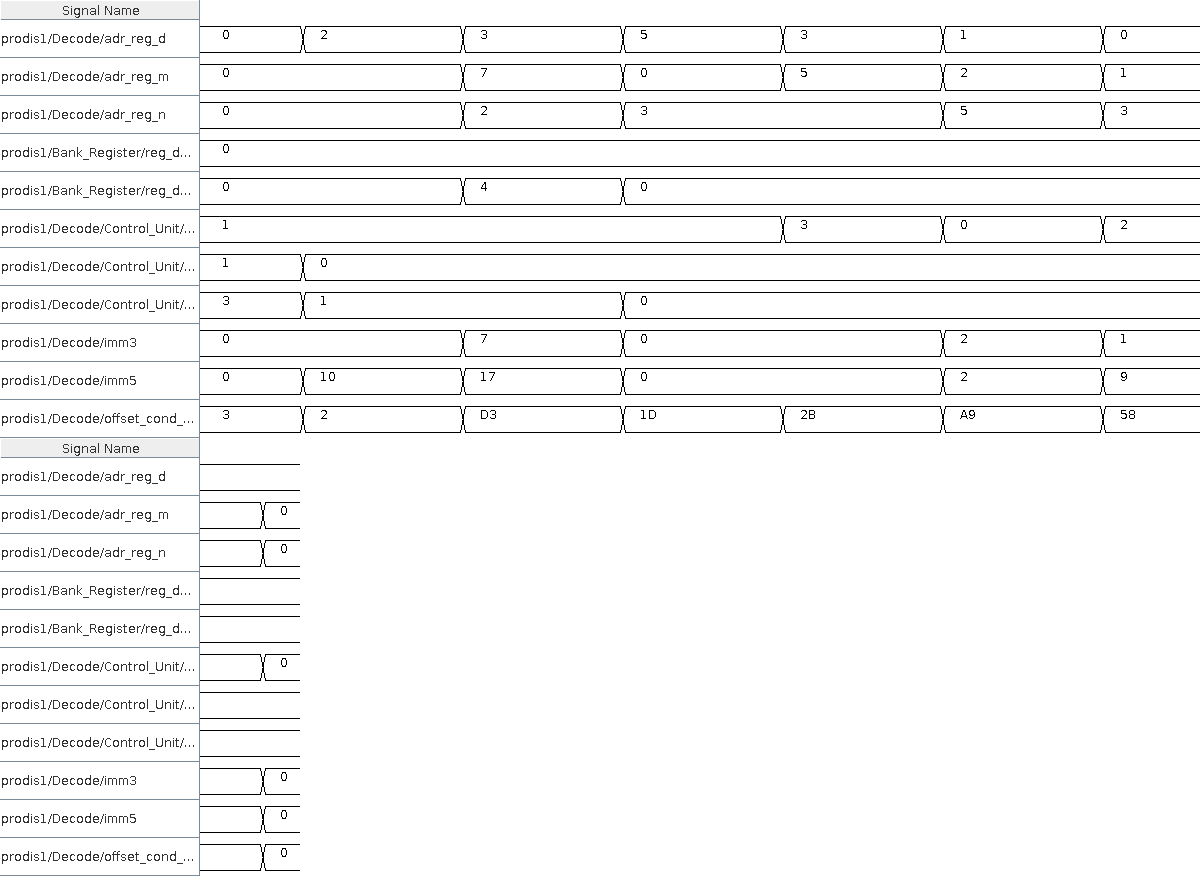
\includegraphics[width=1\textwidth]{src/CHRONO_ETAPE1.png}
    \captionof{figure}{Chronogramme}
    \label{fig:Chronogramme}
\end{figure}
\paragraph{Signaux dans l'ordre:}
\begin{itemize}
    \item     adr\_reg\_d/n/m: adresse des registres (bloc DECODE)
    \item     reg\_data\_out\_m/n: données des registres source (bloc BANK\_REGISTER)
    \item     sel\_op\_alu: operation à effectuer dans l'ALU (bloc DECODE)
    \item     sel\_op\_1/2: placement des opérandes (bloc DECODE)
    \item     imm3/5/8: valeurs immédiates (bloc DECODE)
\end{itemize}
\subsection{Etape 2}
L'objectif de cette étape était de réaliser un circuit permettant de traiter les informations mentionnées dans l'étape 1.
Un bus d'instruction donne les informations nécessaires au fonctionnement du bloc EXECUTE (numéros de registres, type d'opérations à faire, opérandes à utiliser). Le format de ces information est sur 23 bits et se présente comme suit: \medskip \\
\begin{itemize}
\item{[0-2] = sel\_op\_shift}
    \subitem 000: Bypass du bloc
    \subitem 001: Operand 1 shift arithmétique à droite avec Operand 2
    \subitem 010: Operand 1 shift logique à gauche avec Operand 2
    \subitem 011: Operand 1 shift logique à droite avec Operand 2
    \subitem 100: Operand 1 shift rotatif à droite avec Operand 2
\item{[3-6] = sel\_op\_ali}
    \subitem 0000: Bypass du bloc (Operand 1 en sortie)
    \subitem 0001: Operand 1 + Operand 2
    \subitem 0010: Operand 1 - Operand 2
    \subitem 0011: Operand 1 AND Operand 2
    \subitem 0100: Operand 1 OR Operand 2
    \subitem 0101: Operand 1 XOR Operand 2
    \subitem 0110: NOT Operand 1
    \subitem 0111: Operand 1 AND (NOT Operand 2)
    \subitem 1000: Operand 1 * Operand 2
\item{[7-8] = sel\_operand\_2}
    \subitem 00: reg\_data\_out\_m
    \subitem 01: immediate3
    \subitem 10: not used
    \subitem 11: immediate8
\item{[9-10] = sel\_operand\_1}
    \subitem 00: reg\_data\_out\_n
    \subitem 01: 0x0000
    \subitem 10: Branch with link
    \subitem 11: not used
\item{[20] = sel\_shift}
    \subitem 0 : immediate5 
    \subitem 1 : reg\_data\_out\_m 
\end{itemize}

\subsubsection{Liste des blocs Logisim réalisés pour cette étape:}
\begin{itemize}
    \item COMP\_INST: intruction de comparaison
    \item LSL\_INST: shift logique à gauche
    \item ADD\_INST: addition
    \item SUB\_INST: soustraction
    \item ALU: Arithmetic Logic Unit (unité arithmétique et logique)
    \item EXECUTE: bloc principal

\end{itemize}
\subsubsection{COMP\_INST} \label{comp_inst}
\begin{figure}[H]
    \centering
    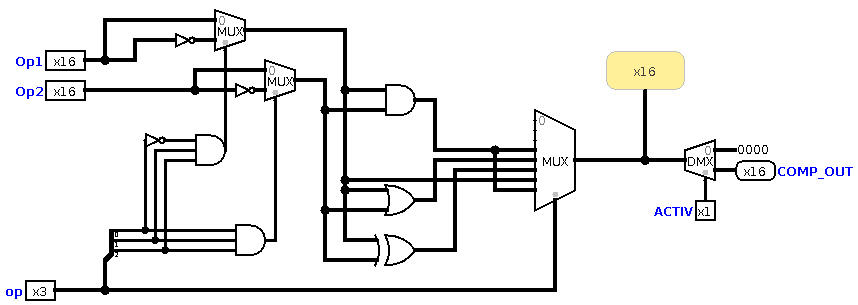
\includegraphics[width=1\textwidth]{src/COMP_INST.png}
    \captionof{figure}{Comparateur logique}
    \label{fig:comp_inst_pic}
\end{figure}
\paragraph{Définition des entrées:}
\begin{itemize}
    \item     op: instruction à effectuer
    \item     Op1: opérande 1
    \item     Op2: opérande 2
    \item     ACTIV: est à 1 lorsqu'il faut effectuer l'opération
\end{itemize}

\paragraph{Définition des sorties:}
\begin{itemize}
    \item     COMP\_OUT: résultat de la comparaison
\end{itemize}
\medskip
Ce bloc permet d'effectuer les comparaisons logiques AND, OR, XOR, NOT(op1) et AND NOT(op2). Seuls les bits [2..0] de \textbf{sel\_op} sont pertinents pour déterminer quelle opération il faut effectuer, puisque le bit 3 est toujours à 0. Un multiplexer permet de renvoyer la comparaison définie par l'op. Deux multiplexer permettent de choisir le NOT de chaque opérande lorsqu'il y a l'instruction NOT et l'instruction AND NOT, et ainsi réutiliser le porte logique AND ou prendre directement la sortie du multiplexer. Tant qu'\textbf{ACTIV} n'est pas à 1, la sortie sera à 0x0000.

\subsubsection{LSL\_INST}
\begin{figure}[H]
    \centering
    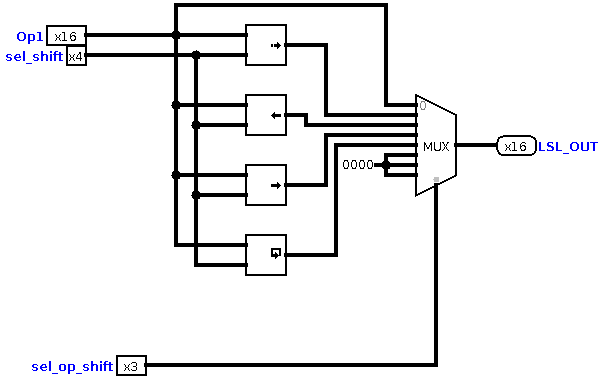
\includegraphics[width=.8\textwidth]{src/LSL_INST.png}
    \captionof{figure}{Shift logique à gauche}
    \label{fig:lsl_inst_pic}
\end{figure}
\paragraph{Définition des entrées:}
\begin{itemize}
    \item     Op1: opérande
    \item     sel\_shift: nombre de bits à décaler
    \item     sel\_op\_shift: indique le type de shift
\end{itemize}

\paragraph{Définition des sorties:}
\begin{itemize}
    \item     LSL\_OUT: résultat du shift logique
\end{itemize}
\medskip
Un shift logique va être effectué dans ce bloc, selon le \textbf{sel\_op\_shift} (voir le détail du bus d'instruction présenté au début de cette étape). Un multiplexer placé en fin du circuit permet de choisir le shift à partir de cette entrée. Les bits [7-5] du MUX sont inutilisés, raison pour laquelle une constante à 0x0000 y a été mise en entrée. L'\textbf{sel\_shift} va permettre de déterminer de combien de bits le décalage doit être fait.

\subsubsection{ADD\_INST}
\begin{figure}[H]
    \centering
    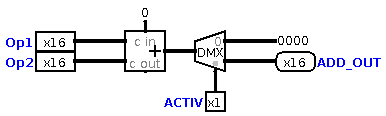
\includegraphics[width=.8\textwidth]{src/ADD_INST.png}
    \captionof{figure}{Addition}
    \label{fig:add_inst_pic}
\end{figure}
\paragraph{Définition des entrées:}
\begin{itemize}
    \item     Op1: opérande 1
    \item     Op2: opérande 2
    \item     ACTIV: est à 1 lorsqu'il faut effectuer l'opération
\end{itemize}

\paragraph{Définition des sorties:}
\begin{itemize}
    \item     ADD\_OUT: résultat de l'addition
\end{itemize}
\medskip
Une simple addition est effecutée entre les opérandes. Tant qu'\textbf{ACTIV} n'est pas à 1, la sortie sera à 0x0000.


\subsubsection{SUB\_INST}
\begin{figure}[H]
    \centering
    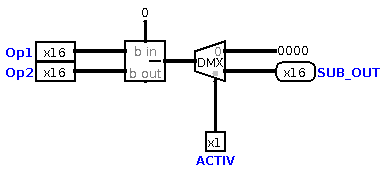
\includegraphics[width=.8\textwidth]{src/SUB_INST.png}
    \captionof{figure}{Soustraction}
    \label{fig:sub_inst_pic}
\end{figure}
\paragraph{Définition des entrées:}
\begin{itemize}
    \item     op: instruction à effectuer
    \item     Op1: opérande 1
    \item     Op2: opérande 2
    \item     ACTIV: est à 1 lorsqu'il faut effectuer l'opération
\end{itemize}

\paragraph{Définition des sorties:}
\begin{itemize}
    \item     SUB\_OUT: résultat de la soustraction
\end{itemize}
\medskip
Une simple soustraction est effectuée entre les opérandes. Tant qu'\textbf{ACTIV} n'est pas à 1, la sortie sera à 0000.

\subsubsection{ALU} \label{alu}
\begin{figure}[H]
    \centering
    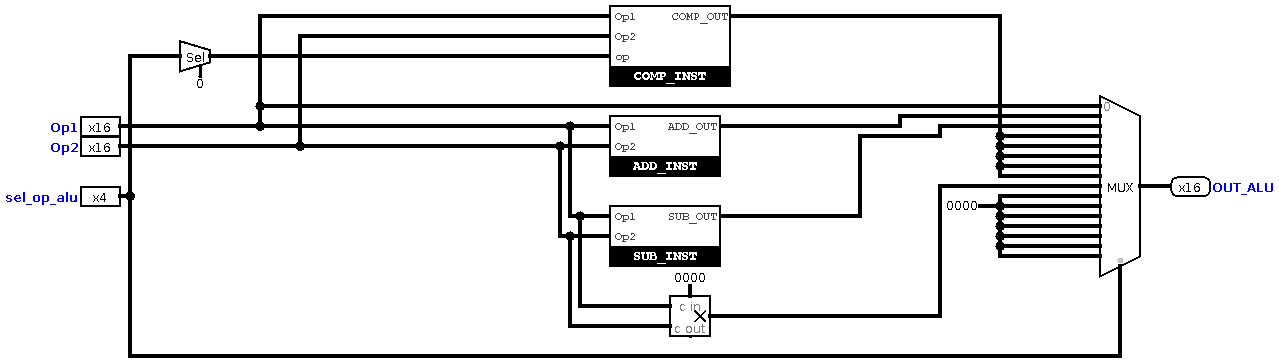
\includegraphics[width=1\textwidth]{src/ALU.png}
    \captionof{figure}{ALU}
    \label{fig:alu_pic}
\end{figure}
\paragraph{Définition des entrées:}
\begin{itemize}
    \item     sel\_op\_alu: instruction à effectuer
    \item     Op1: opérande 1
    \item     Op2: opérande 2
\end{itemize}

\paragraph{Définition des sorties:}
\begin{itemize}
    \item     OUT\_ALU: résultat de l'opération effectuée dans l'ALU
\end{itemize}
\medskip
Les deux opérandes sont reliées à chaque bloc effectuant les instructions, afin de leur tranmettre les données nécessaires. L'entrée \textbf{sel\_op\_alu} correspond aux bits [3-6] du bus d'instructions, et va, selon sa valeur, permettre de déterminer quelle est l'instruction qui doit être effectuée.\\
\smallbreak
\begin{tabular}{|c|c|}
    \hline
        Opcode & Bloc \\
        \hline
        0000   & Bypass (Op1) \\
        \hline
        0001   & ADD\\
        \hline
        0010   & SUB \\
        \hline
        0011   & COMP (AND) \\
        \hline
        0100   & COMP (OR) \\
        \hline
        0101   & COMP (XOR) \\
        \hline
        0110   & COMP (NOT Op1) \\
         \hline
        0111   & COMP (AND) \\
        \hline
        1000   & Multiplication\\
        \hline    
\end{tabular}
\subsubsection{EXECUTE} \label{execute}
\begin{figure}[H]
    \centering
    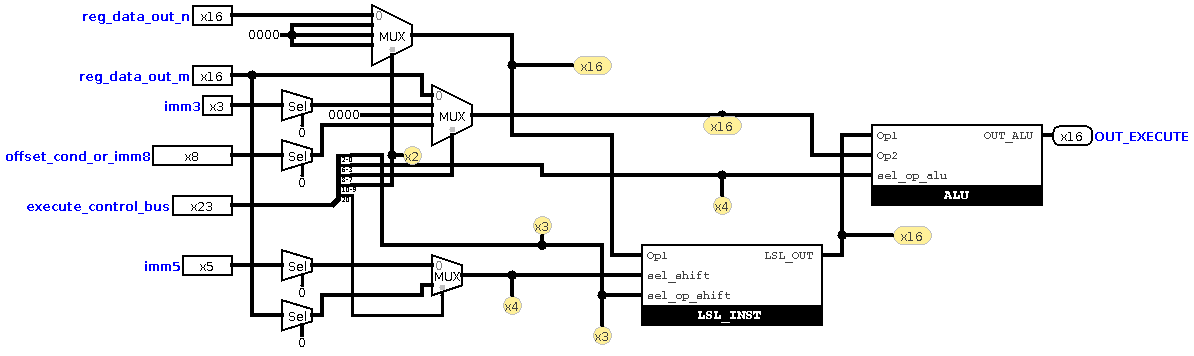
\includegraphics[width=1\textwidth]{src/EXECUTE.png}
    \captionof{figure}{EXECUTE}
    \label{fig:execute_pic}
\end{figure}
\paragraph{Définition des entrées:}
\begin{itemize}
    \item     reg\_data\_out\_n: données du registre source 1
    \item     reg\_data\_out\_m: données du registre source 2
    \item     imme3, imme5, imme8: valeurs immédiates
    \item     execute\_control\_bus: bus d'instruction
\end{itemize}

\paragraph{Définition des sorties:}
\begin{itemize}
    \item     OUT\_EXECUTE: résultat des opération effectuées dans EXECUTE et dans l'ALU
\end{itemize}
\medskip
La partie EXECUTE va prendre en entrée toutes le bus d'instruction qui va permettre de déterminer les différentes instructions à effecuter. Il est séparé comme présenté au début d'étape 2.
La structure de ce circuit sera décrite à partir de ses entrées, et selon les difféntes séparations de bits du bus de contrôle, dont les valeurs vont déterminer les entrées à utiliser.
\textbf{reg\_data\_n} va être utilisée seulement lorsque les bits [10-9] sont à 00. Les autres valeurs en sortie du MUX sont toutes à 0, d'où la constante. La sortie de ce bus correspond à l'opérande 1 à mettre en entrée du shift logique (qui va donc subir le shift).
Les entrées \textbf{reg\_data\_m}, \textbf{imm3} et \textbf{imm8} vont être déterminées par les bits [8-7] du bus d'intructions. Ainsi, ils se retrouvent en entrée d'un même multiplexer. La valeur 10 en bits [8-7] du bus n'est pas utilisée, ainsi, il y a une constante à 0. Comme la sortie de ce MUX correspond à l'opérande 2 (en entrée de l'ALU), un bit selector va permettre d'étendre les valeurs de \textbf{imm3} et \textbf{imm8} sur 16 bits.
Reste \textbf{imm5}, dans un MUX avec \textbf{reg\_data\_m}. Seuls 4 bits de ces deux entrées sont sélectionnées, car elles déterminent le \textbf{sel\_shift} du shift logique, c'est-à-dire le nombre de bits qu'il faut décaler, qui est sur 4 bits. La valeur du MUX est déterminée par le  bit [20] du bus d'instructions. Restent les bits [2-0] du bus d'instructions, qui sont en entrée  \textbf{shel\_op\_shift} du shift logique, et vont déterminer le type de shift logique à effectuer. La sortie du shift logique correspond à l'opérande 1 de l'ALU. Enfin, les bits [6-3] du bus d'instructions sont en entrée \textbf{sel\_op\_alu} de l'ALU, et permettent de choisir l'opération à effectuer dans l'ALU.
\subsection{Etape 3}
L'objectif de cette partie était de modifier le circuit afin qu'il puisse traiter des informations supplémentaires précisées dans la donnée, à savoir:
\medskip

\begin{itemize}
    \item Shift logique à gauche, avec valeur immédiate
    \item Shift logique à gauche, avec valeur en registre
    \item Shift logique à droite, avec valeur immédiate
    \item Shift logique à droite, avec valeur en registre
    \item Opération logique AND
    \item Opération logique OR
    \item Opération logique XOR
    \item Opération logique NOT
    \item Addition avec valeur immédiate
    \item Addition avec valeur en registre
    \item Soustraction avec valeur immédiate
    \item Soustraction avec valeur en registre
\end{itemize}
L'étape 3 a été réalisée simultanément avec l'étape 2, puisqu'il d'agissait de permettre au circuit de traiter des informations qui étaient aussi en rapport avec cette étape. Ainsi, il faut se référer à l'étape 2.

\subsubsection{Chronogramme}
\begin{figure}[H]
    \centering
    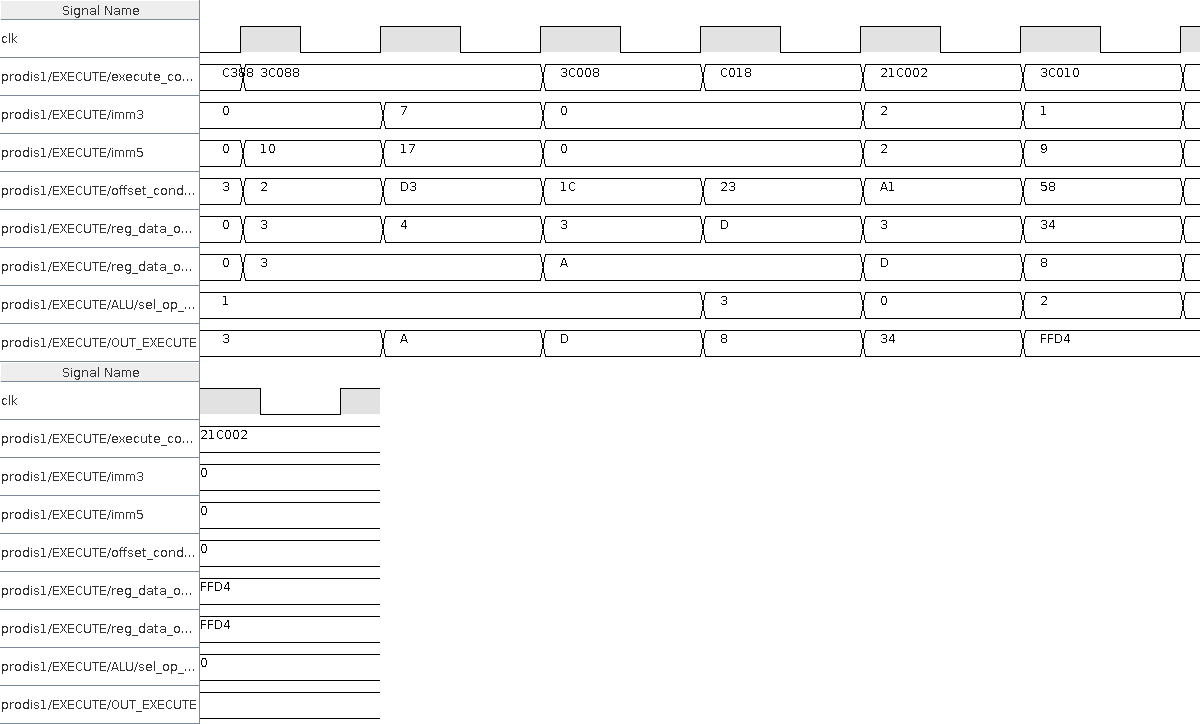
\includegraphics[width=1\textwidth]{src/CHRONO_FINAL.png}
    \captionof{figure}{Chronogramme}
    \label{fig:chrono_final_pic}
\end{figure}
\paragraph{Signaux dans l'ordre:}
\begin{itemize}
    \item     clk: horloge
    \item     execute\_control\_bus: bus d'instructions (bloc EXECUTE)
    \item     imme3, imme5, imme8: valeurs immédiates (bloc EXECUTE)
    \item     reg\_data\_out\_m/n: données des registres source (bloc EXECUTE)
    \item     sel\_op\_alu: operation à effectuer dans l'ALU (bloc ALU)
    \item     OUT\_EXECUTE: valeur en sortie (bloc EXECUTE)
\end{itemize}
\section{Conclusion}
Ce laboratoire nous a permis de comprendre la partie EXECUTE d'un processeur, et de faire le lien avec les deux parties FETCH et DECODE que nous avions vues dans les deux laboratoires précédents.\\
Nous avons eu de la peine au début pour savoir comment interconnecter les choses entre elles, mais une fois ce problème réglé, la suite était relativement intéressante et nous a permis de comprendre encore mieux le fonctionnement global d'un telle circuit.

\end{document}